The given system of equations \eqref{eq:solutions/det/53/1} can be written the matrix equation form as
\begin{align}
    \vec{A}\vec{x}=\vec{b}\\
    \label{A}
    \implies \myvec{2&-1\\1&1}\myvec{x\\y}=\myvec{5\\4}
\end{align}
The augmented matrix for \eqref{A} is row reduced as follows
\begin{align}
    \myvec{2&-1&5\\1&1&4}\\
    \xleftrightarrow[]{R_2\leftarrow \frac{2R_2-R_1}{3}}
    \myvec{2&-1&5\\0&1&1}\\
    \xleftrightarrow[]{R_1\leftarrow \frac{R_1+R_2}{2}}
    \myvec{1&0&3\\0&1&1}\\
    \implies Rank\myvec{2&-1\\1&1}=Rank\myvec{2&-1&5\\1&1&4}
    \\=1 < dim\myvec{2&-1\\1&1}
\end{align}
Hence \eqref{eq:solutions/det/53/1} is consistent and has unique solution \myvec{3\\1}\\
\begin{figure}[!ht]
\centering
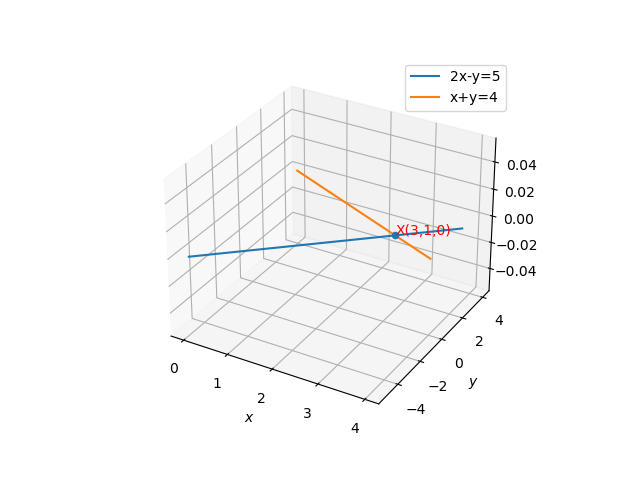
\includegraphics[width=\columnwidth]{./solutions/det/53/Plot_3D.png}
\caption{Intersection of lines 2x-y=5 and x+y=4}
\label{fig1solutions/det/53/}
\end{figure}
